\section{Planarity}
\label{section:planar-graphs}
A fascinating and important class of graphs that we will focus on in \Cref{chapter:network-diversion} are \emph{planar graphs}. We will give the most important definitions and facts about planar graphs here, and refer the reader to \cite{source:planar_graphs} if they wish to read more.

\subsection{Planar embeddings}
\begin{definition}[Embedding]
    Let $G$ be a graph. An \emph{embedding} of $G$ is a drawing of $G$ on the plane $\mathbb{R}^2$, with points representing vertices and curves representing edges between their endpoints' respective points, such that none of the edges intersect each other except in their endpoints.
\end{definition}

\begin{definition}[Planar graph]
    We say that a graph $G$ is a \emph{planar graph} if there exists a planar embedding of $G$. A planar graph along with a specific planar embedding is called a \emph{plane graph}.
\end{definition}

Many real-life graphs, especially those based on physical structures, are either planar or almost so. Two edges crossing often entails an inefficiency or extra cost: like having to build a bridge over a road instead of joining the two roads in a crossroad. Many algorithmic problems are much easier to solve in planar graphs, and they are common enough in practical use that the restriction is not too restrictive to be useful.

\begin{definition}[Straight-line embedding]
    Let $G$ be a graph. A \emph{straight-line embedding} of $G$ is a planar embedding of $G$ where each edge can be drawn as a line segment between its endpoint vertices and still not cross any other edge. In a straight-line embedding, we can forgo the mappings of the edges altogether and consider the mapping of vertices only. Such embeddings always exist: if $G$ is planar then there is a straight-line embedding of $G$.
\end{definition}

See \Cref{subfigure:k4-a}, \Cref{subfigure:k4-b} and \Cref{subfigure:k4-c} for an example of a planar graph. \Cref{subfigure:k4-a} and \Cref{subfigure:k4-c} also show planar embeddings of the graph. \Cref{subfigure:k33} shows a graph that is not planar, since no planar embeddings of the graph exist. Note that in all these examples we have drawn all the edges as straight line segments, but that is not necessary: as long as a curve does not cross any other curves it can be as curved as we want.

\begin{figure}
    \centering
    \begin{subfigure}{.23\textwidth}
        \centering
        \includesvg{figures/k33.svg}
        \caption{Not planar}
        \label{subfigure:k33}
    \end{subfigure}\hfill%
    \begin{subfigure}{.23\textwidth}
        \centering
        \includesvg{figures/k4-a.svg}
        \caption{Planar}
        \label{subfigure:k4-a}
    \end{subfigure}\hfill%
    \begin{subfigure}{.23\textwidth}
        \centering
        \includesvg{figures/k4-b.svg}
        \caption{Planar, it is the same graph as in \Cref{subfigure:k4-a}}
        \label{subfigure:k4-b}
    \end{subfigure}\hfill%
    \begin{subfigure}{.23\textwidth}
        \centering
        \includesvg{figures/k4-c.svg}
        \caption{Planar, with colored faces.}
        \label{subfigure:k4-c}
    \end{subfigure}
    \caption{Examples of planar and non-planar graphs}
\end{figure}

It is generally complicated to determine whether a given graph is planar in practice and to compute an appropriate embedding if it is. For all the algorithms we have implemented in this paper, if they take a planar graph as input, we have for simplicity assumed that we are also given a planar embedding of the graph. Furthermore, since all planar graphs also have straight-line embeddings, we have assumed that the given embeddings are straight-line embeddings. Our theoretical results hold for planar graphs in general, but in practice, these assumptions make implementing the algorithms less tedious.

\subsection{Duality}
The next topic is easy to visualize and understand, but challenging to formalize. Imagine loading a drawing of a planar graph like the one in \Cref{subfigure:k4-a} into an image editing program, and using the fill tool to cover each region in a different color, like in \Cref{subfigure:k4-c}. Each such region is called a \emph{face} of the graph, including the region 'outside' the graph called the \emph{outer} face. Two faces are adjacent if they are separated by just a single edge: if we were to delete the edge our fill tool would give both the same color. We will now formalize this concept.

\begin{definition}[Face]
    Let $G$ be a plane graph. A \emph{face} of $G$ is a region in the embedding bounded by a cycle that contains no other vertices or edges. Equivalently, we can define faces as the connected components that remain in $\mathbb{R}^2$ after we delete all vertices and edges from our embedding. 

    Note that different embeddings of the same planar graph may yield different faces. When we refer to a face in a graph, it is always in relation to a certain embedding of the graph.
\end{definition}

\begin{definition}[Duality of planar graphs]
    Let $G$ be a plane graph. The \emph{dual graph} of $G$, denoted as $G^\star$, is the graph where 
    \begin{itemize}
        \item The vertices represent faces of $G$
        \item There is an edge between two faces if they are adjacent in $G$.
    \end{itemize}
\end{definition}

Each edge in $e \in E(G)$ will always have a face on either side, possibly the same face, and thus have a corresponding edge $e^\star \in E(G^\star)$ in the dual graph. We can therefore define two convenience functions $\leftt, \rightt~: E(G) \rightarrow V(G^\star)$ to get the left and right faces of an edge, respectively. If $G$ is weighted, we usually set the weights of $E(G^\star)$ according to their counterparts: $\weight(e^\star)~:= \weight(e)$. See \Cref{subfigure:k4-with-dual} for an example of a dual graph.

Note that the dual graph is also planar, and the dual of the dual is the original graph\footnote{Strictly speaking, there is an embedding of $G^\star$ such that $G^{\star\star} \cong G$.}. We could then for example let $e$ be an edge in the dual graph, and then refer to its real counterpart as $e^\star$. It would not be wrong, but it could possibly lead to confusion. Furthermore, we do not need that fact for any of the results in this thesis. We will therefore give variable names like $G$, $u$, and $e$ for the graphs, vertices, and edges that we are 'working on', and use variable names like $G^\star$, $u^\star$ and $e^\star$ for their dual equivalents only in intermediary computations before arriving at results for our original graph.

\begin{fact}[Cycle--cut duality]
\label{fact:dual-cycle-is-real-cut}
    Let $G~:= (V, E, from, to)$ be a connected planar graph, and let $C^\star$ be a simple cycle in $G^\star$. Then $C^\star$ will always correspond to a minimal cut in $G$. If we define $C~:= \{e ~ | ~ e^\star \in E(G^\star)\}$ as the edges in $E(G)$ that correspond to edges in $C^\star$, then $(V,E \setminus C, \from, \too)$ is a disconnected graph of exactly two components. If the cycle $C^\star$ is not simple, then we still end up with a disconnected graph, but we may have more than just two components.

    See \Cref{figure:cycle-cut} for an example. In \Cref{figure:dual-with-cycle} we have found a simple cycle in the dual graph, and if we delete the corresponding edges in the original graph we end up with the disconnected graph in \Cref{subfigure:k4-cut}.
\end{fact}

\begin{figure}[h]
    \centering
    \begin{subfigure}{.3\textwidth}
        \centering
        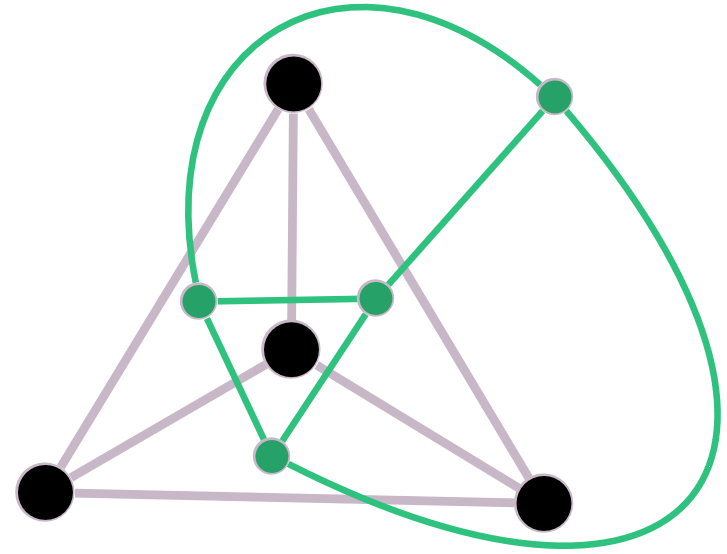
\includegraphics[width=4cm]{figures/duality/k4 with dual.png}
        \caption{A planar graph with its dual colored in green}
        \label{subfigure:k4-with-dual}
    \end{subfigure}\hfill%
    \begin{subfigure}{.3\textwidth}
        \centering
        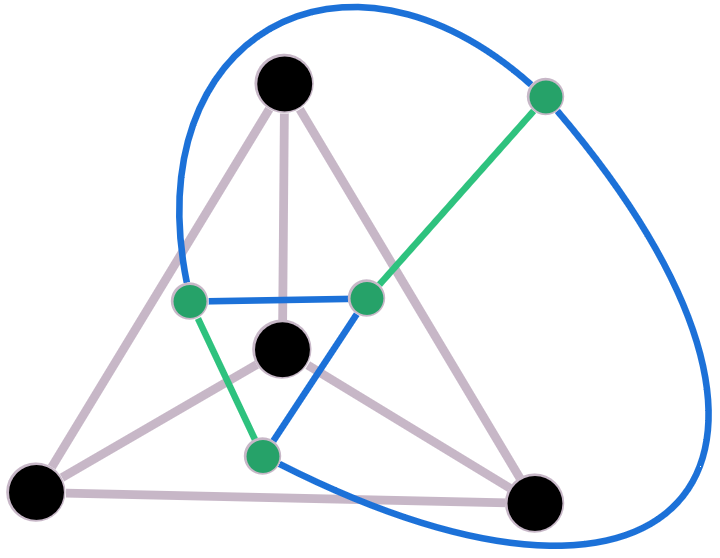
\includegraphics[width=4cm]{figures/duality/dual with cycle.png}
        \caption{A simple cycle in the dual, colored in blue}
        \label{figure:dual-with-cycle}
    \end{subfigure}\hfill%
    \begin{subfigure}{.3\textwidth}
        \centering
        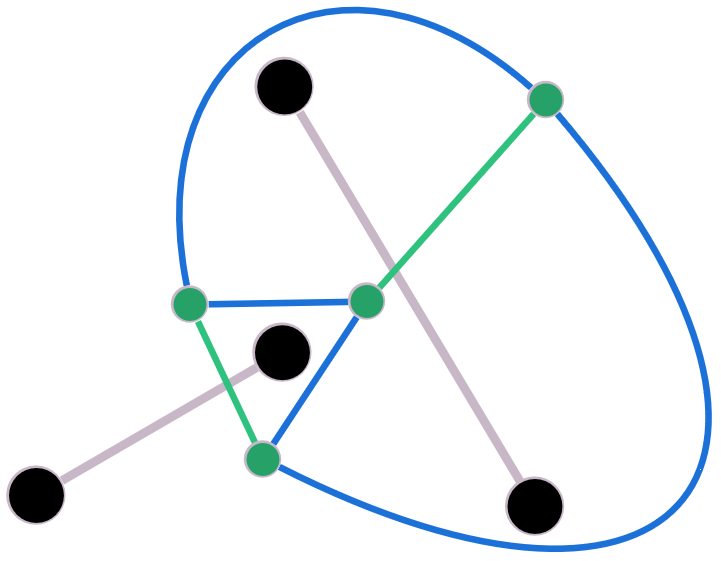
\includegraphics[width=4cm]{figures/duality/k4 cut in pieces.png}
        \caption{Deleting the edges that cross the dual's cycle cuts the graph in two}
        \label{subfigure:k4-cut}
    \end{subfigure}
    \caption{A simple cycle in a dual graph always corresponds to a cut in the original graph.}
    \label{figure:cycle-cut}
\end{figure}

\begin{theorem}[The relation between the number of vertices, edges and faces]
    Let $G~:= (V, E, \from, \too)$ be a connected planar graph, where $n~:= |V|, m~:= |E|$, and $f$ is the number of faces in any embedding of $G$. \\
    Claim: $n + f - m = 2$.

    \begin{proof}
        Let $H \sqsubseteq G$ be any non-empty connected subgraph that does not have any cycles, and let $n_H~:= |V(H)|$. Since it does not have any cycles, we have that:
        \begin{itemize}
            \item The outside face must be the only face: $f_H~:= 1$.
            \item Each edge must connect a 'new' vertex to the rest of the graph, except the first edge which connects two new vertices. Therefore the number of edges is one less than the number of vertices: $m_H~:= n_H - 1$.
        \end{itemize}
        We now have that $n_H + f_H - m_H = n_H + 1 - (n_H-1) = 2$, so the equality holds for this subgraph.

        Now we can iteratively add either an edge alone or both a vertex and an edge to $H$ until we have $G$. If we add just an edge, we increase both $m_H$ and $f_H$ by 1, and the equality still holds. If we add a new vertex with a new edge, we increase both $n_H$ and $m_h$ by one, and the equality still holds. 
        
        Therefore, the equality $n + f - m = 2$ holds for any connected planar graph $G$.
    \end{proof}
\end{theorem}

\begin{corollary}
    The number of faces is fixed. A graph may have different faces depending on the embedding, but the number of faces is always the same.
\end{corollary}
    
\begin{corollary}
    \label{corollary:m-leq-3n}
    Since all faces (except possibly the outer face) are bounded by at least three edges, and all edges touch at most two faces, we can show that if $n \geq 3$, then $m \leq 3n-6$.
\end{corollary}
